\subsubsection{Proposed solution}\label{proj_manip}

There are several industrial manipulators which fulfill the HVOF
requirements. Companies as Fanuc, Motoman, ABB and KUKA, for example,
manufacture manipulators compatible with the bottom hatch dimensions and HVOF
requirements, and workspace that the entire turbine blade could be coated at a
fixed base position. However, those manipulators are too big to operate behind
the blade, on the distributor side, due to environment collision, joint
constraints, and robot manipulability. Besides, manipulators with such
workspace are heavyweight, thus the robot placement and motion would be complex
inside the Runner area. A feasible solution would be to select a mid-sized
manipulator and made a rail base to place and move the robot.

%Há diversos manipuladores robóticos industriais com as especificações
%necessárias para a realização da tarefa de metalização por HVOF. As empresas
%Fanuc, Motoman, ABB e KUKA fabricam manipuladores com dimensões compatíveis com
% o acesso pela escotilha inferior e velocidade, precisão, e espaço de trabalho que
%cumprem os requisitos para a execução do processo em todo um lado da pá, em uma
%base fixa. Porém, há incompatibilidade atrás da pá e a necessidade de escolher
% a posição correta do manipulador em relação à pá, a fim de maximizar a sua área de trabalho, no ambiente da
%turbina, o que pode restringir os seus movimentos.
%Como as pás podem ser giradas até um ângulo de $14.5^o$, são discutidas as
% ideias de posicionamento do manipulador entre as pás, a fim de executar a operação em ambos os lados da
%pá (um lado de cada pá), e o posicionamento fixo à frente e depois atrás à pá.

The base consists of a transport rail and a positioning rail, both fixed
in the Runner area by magnetic coupling and/or welding. The first solves a
logistic problem, as it starts at the bottom hatch entry and goes to the blade,
moving the robot through the Runner area. The latter is coupled to the main rail and positions the robot close to the
blade, enabling displacement along it, solving the horizontal HVOF cover of the
blade.

The base may be summarized in three joints: prismatic (main rail), revolution
(joint between main and second rail), and prismatic (second rail) (P-R-P). As
the robot can not vertically cover the entire blade, there is still the need of
different vertical positions, which should be manually selected. The blade can
be coated on linear or circular motion, and, in both cases, the manipulator will
be responsible for speed, position and gun orientation. The solution for gun
direction exchange (\textit{long stop}) is an actuated valve to redirect the
coating particles.

%A base por um trilho de transporte e um de posicionamento. Ambos são fixados no
%aro câmara por acoplamentos magnéticos e/ou solda. O primeiro começa na
%entrada da pá e vai até a pá, permitindo o deslocamento do robô pelo aro
% câmara.
%O último é acoplado ao trilho principal e posiciona o robô próximo a pá, além
% de possibilitar o deslocamento ao longo desta. Dessa forma, a base pode ser
%resumida em três juntas: prismática, revolução e prismática (PRP). Como o robô
%não possui alcance de toda a pá, há, ainda, a necessidade de posições verticais
%diferentes escolhidas manualmente. A pá pode ser processada em movimentos
%circulares ou lineares e, em ambos os casos, o manipulador ficará responsável
% pela velocidade, posição e orientação do processo. A troca de sentido de movimento deverá ocorrer fora da
%pá, ou devem ser utilizadas placas de sacrifício, ou válvulas para
%redirecionamento das partículas de revestimento.

%Esse tipo de abordagem simplifica a movimentação do robô no
%trilho, uma vez que o trilho seria totalmente reto, e possibilitaria a
%metalização de um dos lados das quatro pás com uma única instalação de base.
%Porém, mesmo nesta solução, a altura do trilho deverá ser ajustada três vezes
% para cada lado de pá.


%Em ambos os sistemas propostos, é necessária a implementação de um sistema de
%localização do robô em relação à pá, tornando possível a geração de um
%planejamento de trajetórias para o processo de metalização. O sistema de
%localização pode ser concebido por sensores externos
%ao robô (câmeras e outros), ou instalados no próprio manipulador/base.


%The alternative to avoid contact with the blade consists of a single rail
%rectilinear fixed by magnetic bases or welding of the rim in the soil chamber.
% Like the robot has not reach all the shovel, there is still a need positions
%different vertical. The blade can be processed in circular movements or
%linear and, in both cases, the handler will be responsible for the speed,
%position and orientation of the process. The exchange direction of movement
% should occur outside the shovel or must sacrifice cards used.

%\paragraph{Transport rail}

A mid-sized robot manipulator should be hoisted through the bottom
hatch, placed on a rail base with magnetic holders and carried
to the blade, as in Fig.~\ref{fig::rail1}. At that position, the robot should
switch to the other rail. 
%That strategic position (robot between blades) is
% advantageous as it allows the manipulator to operate adjacent blades without
% rail disassembling or major positioning changes.

\begin{figure}[h!]	
	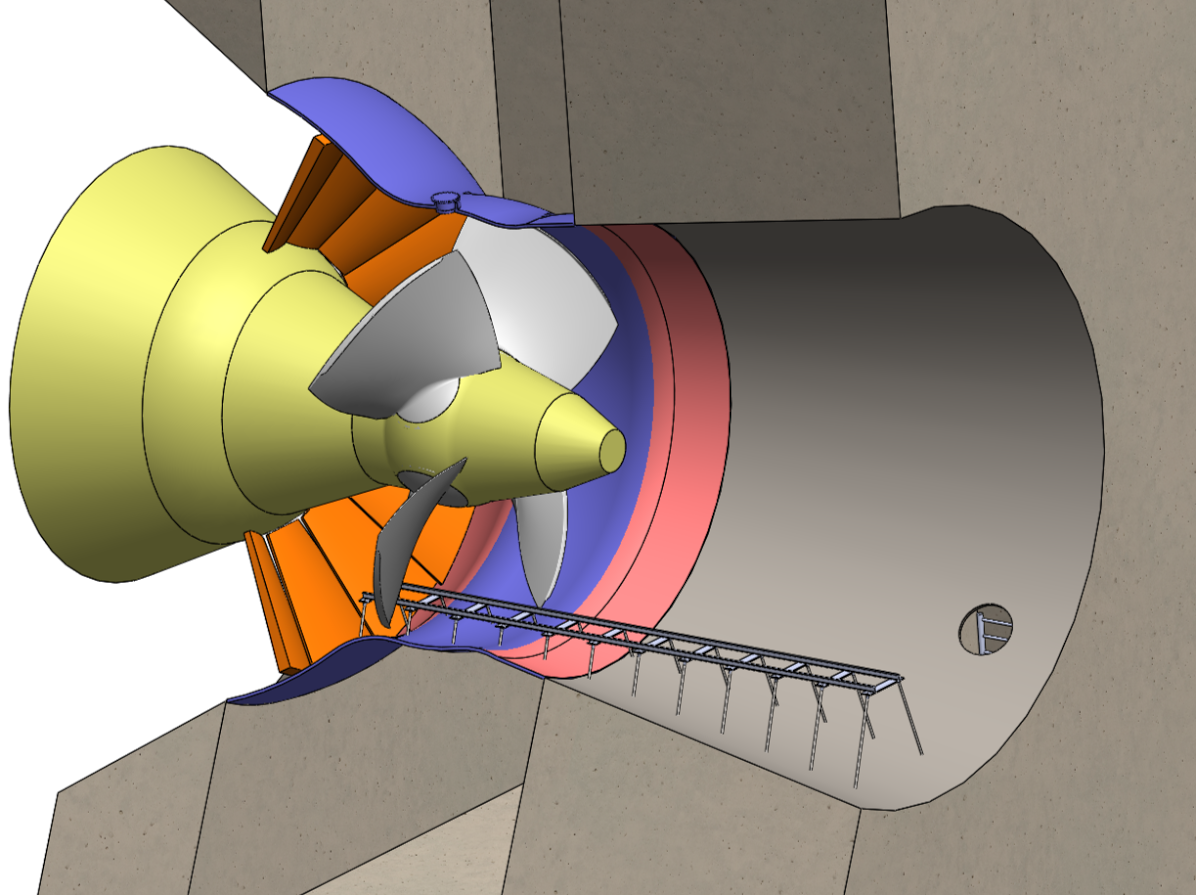
\includegraphics[width=\columnwidth]{figs/manipuladores/rail1.PNG}
	\caption{Transport rail mounted inside the turbine.}
	\label{fig::rail1}
\end{figure}

%A figura~\ref{fig::andaime} mostra o espaço entre as pás da turbina, dentro do
%aro câmara. Um robô manipulador de médio porte pode ser fixado em uma base
%magnética, na posição que se encontra a escada da figura~\ref{fig::andaime}.
%Essa posição é vantajosa por possibilitar a execução da tarefa em duas pás
%(frente de uma e verso da outra), sem desmontar ou fazer grandes alterações no
%posicionamento da base do robô, diminuindo as intervenções e tempo de tarefa.

% However, a purely geometric study shows that the necessary workspace for
% adjacent blades coating, assuming a fixed base between the blades,
% is around 5 m reach. The industrial manipulator IRB5500, for example, developed
% by ABB for painting, and is a large sized manipulator and has 3 meters range,
% 600 kg.
% As no mid-sized industrial robot was found for completely cover
% the blade on a fixed base position, a positioning rail should be made.

%O estudo puramente geométrico demonstra que o alcance do manipulador robótico
%para o processamento de ambos os lados das pás, considerando uma base fixa
% entre as pás, deverá ser em torno de 5 metros. O manipulador industrial IRB5500,
%desenvolvido pela ABB para pintura, possui 3 metros de alcance, porém 180 kg, o
% que já dificulta ou até impossibilita a logística de movimentação e posicionamento in-situ. Não foi encontrado um robô
%industrial com o alcance necessário e que tivesse as dimensões máximas da
%escotilha inferior. 

%A solução conceitual de posicionar um manipulador industrial entre as pás deve
%avaliar, portanto, todas as configurações necessárias da base (orientações e
%posições) para garantir que todo o espaço de trabalho do manipulador mais base
%cubra os lados de ambas as pás. O número de configurações e o projeto
%mecânico da base são necessários para a viabilização da solução,
%uma vez que será possível avaliar as intervenções e complexidades. Bases
%autônomas diminuem o número de intervenções e aumentam a precisção do sistema,
%porém aumentam a complexidade, o custo devido ao número de sensores e
% atuadores, e o peso do sistema, prejudicando a logística.

%\paragraph{Positioning rail}
Fixedly positioning a robotic manipulator with magnetic holders at the front or
at the back of the blade for HVOF process is a natural solution, since it is
similar to the companies procedure. However, a purely geometric
study, using the real dimensions of the blade, shows that the manipulator must
have more than 2.5 m reach for full blade cover. To perform this task, workspace
analysis was conducted to confirm the geometric study and a mid-sized
robot can not reach the entire blade. Therefore, its base should be able to move
horizontally and vertically (Fig.~\ref{fig::rail2}).

\begin{figure}[h!]	
	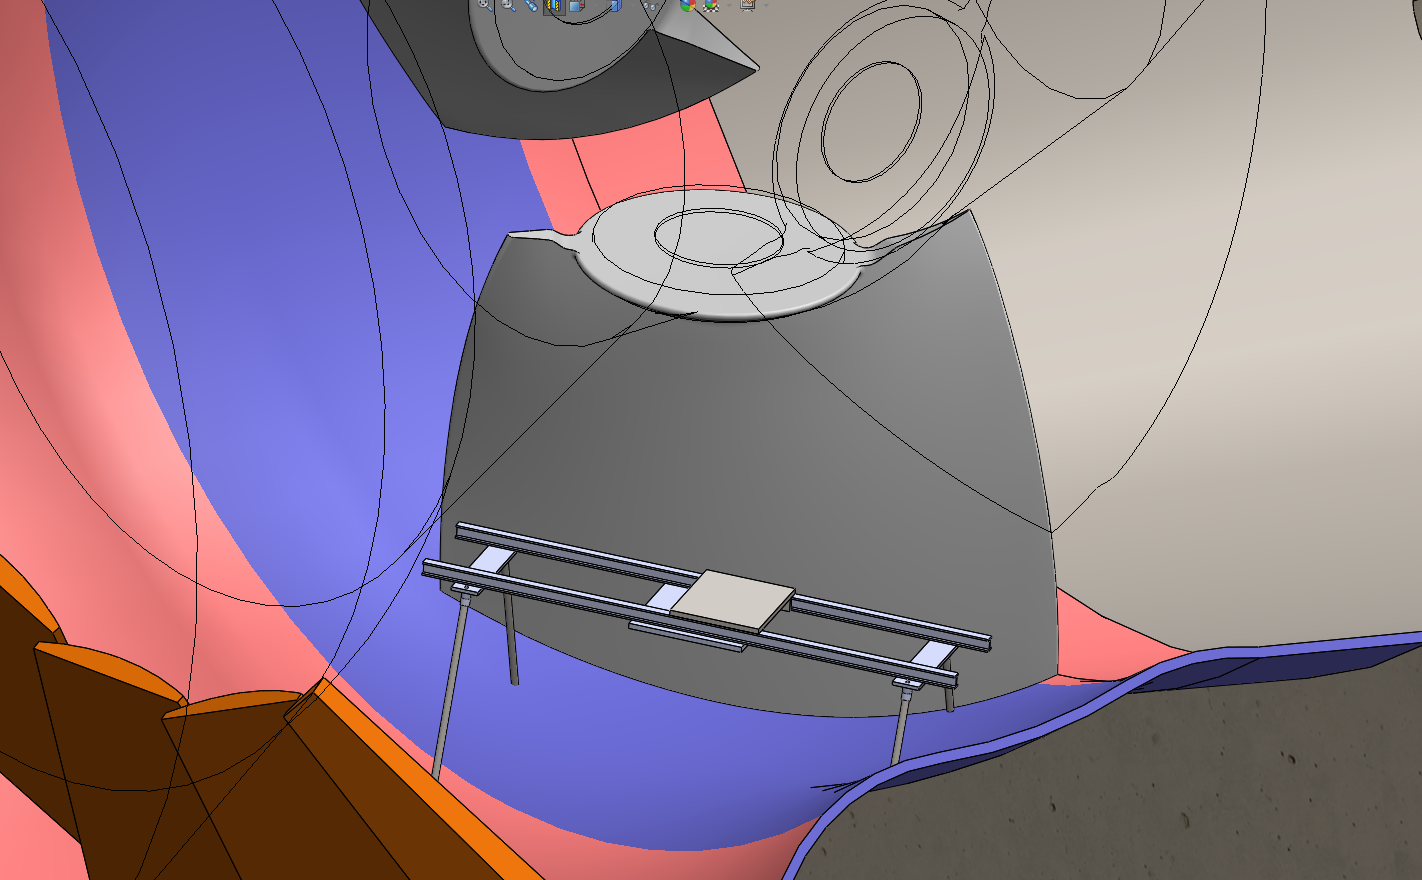
\includegraphics[width=\columnwidth]{figs/manipuladores/rail2.PNG}
	\caption{Positioning rail behind the blade.}
	\label{fig::rail2}
\end{figure}


\paragraph{Solution conclusion}
In terms of robotics, industrial manipulators on a rail base is the simplest
among all solutions for the bottom hatch. There is no mechanical design for the
manipulator, since it will be acquired in one of the aforementioned
manufacturers, but the mechanics will be responsible for the base design (rigid
and modular), the magnetic couplings, and logistics.
